\newpage

\section[Day 8: Convergence \& Cauchy]{ Convergent and Cauchy Sequences }

\subsection{ Convergent Sequences }

    \begin{definition}{Convergent Sequence}{16cm}
        A sequence \{$x_n$\} in metric space X {\color{lblue} converges} if
        there is a x $\in$ X such that:

        \hspace{1cm}
        For every $\epsilon$ $>$ 0, there is a N $\in$ $\mathbb{Z}$ such that
        for all n $\geq$ N, d($x_n$,x) $<$ $\epsilon$
        
        Then, \{$x_n$\} converges to x:
        \hspace{1cm}
        $\lim_{n \rightarrow \infty}$ $x_n$ = x
        \hspace{1cm}
        \{$x_n$\} $\rightarrow$ x

        If \{$x_n$\} does not converge, then it diverges.
    \end{definition}



    \begin{figure}[h]
        \centering
        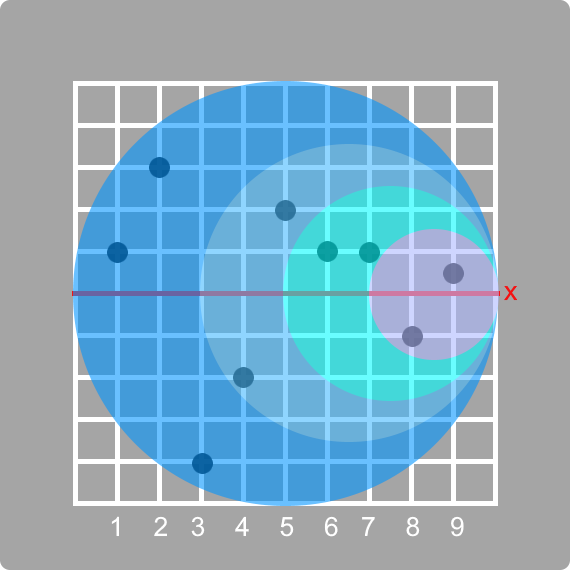
\includegraphics[scale=0.3]{Images/8.1.1.png}
    \end{figure}



    \begin{example}[16cm]
        \begin{enumerate}[label=(\alph*), leftmargin=0.5cm, itemsep=0.1cm]
            \item Let $x_n$ = $\frac{1}{n}$ in $\mathbb{R}^2$.
                Then, $\lim_{n \rightarrow \infty}$ $x_n$ = 0

                { \color{magenta} \underline{Proof} }
    
                \fbox{
                \begin{minipage}{15cm}
                    For $\epsilon$ $>$ 0, there is a $\frac{1}{N}$ $<$ $\epsilon$.
                    Then:
    
                    \hspace{1cm}
                    d($x_n$,0) = $|x_n - 0|$ = $\frac{1}{n}$
                    $<$ $\frac{1}{N}$ $<$ $\epsilon$
                \end{minipage} }
    
            \item Let $x_n$ = $(-1)^n$ + $\frac{1}{n}$ in $\mathbb{R}^2$.
                Then, \{$x_n$\} diverges.
    
                { \color{magenta} \underline{Proof} }
    
                \fbox{
                \begin{minipage}{15cm}
                    $\lim_{n \rightarrow \infty}$ $x_n$
                    = $\lim_{n \rightarrow \infty}$ $(-1)^n$
                    + $\lim_{n \rightarrow \infty}$ $\frac{1}{n}$
                    = $\lim_{n \rightarrow \infty}$ $(-1)^n$
    
                    Since $(-1)^n$ alternates between -1 and 1, then
                    \{$x_n$\} diverges.
                \end{minipage} }
        \end{enumerate}    
    \end{example}

    \vspace{0.5cm}



    \begin{ltheorem}{A convergent sequence is unique and bounded}{1.5cm}
        \item \{$p_n$\} converges to p $\in$ X if and only if
            every N$_r(p)$ contains all, but finitely many $p_n$

            \begin{proof}[15.5cm]
                Suppose $p_n$ $\rightarrow$ p.
                Then for N$_{\epsilon}(p)$, any q $\in$ X such that
                d(q,p) $<$ $\epsilon$ is q $\in$ N$_{\epsilon}(p)$.
                Since $p_n$ $\rightarrow$ p, there is a N such that for
                n $\geq$ N, d($p_n$,p) $<$ $\epsilon$.
                Thus, for n $\geq$ N, $p_n$ $\in$ N$_{\epsilon}(p)$.

                Suppose every N$_r(p)$ contains $p_n$ for all, but finitely
                many n.

                For $\epsilon$ $>$ 0, let N$_{\epsilon}(p)$ be the set of
                all q $\in$ X such that d(p,q) $<$ $\epsilon$.
                Thus, there exists a N such that $p_n$ $\in$ N$_{\epsilon}(p)$
                if n $\geq$ N.
                Thus, d($p_n$,p) $<$ $\epsilon$ so $p_n$ $\rightarrow$ p.
            \end{proof}

        \item If p,p' $\in$ X and \{$p_n$\} converges to p and p', then p = p'

            \begin{proof}[15.5cm]
                For $\epsilon$ $>$ 0, there exists N,N' such that:

                \hspace{1cm}
                d($p_n$,p) $<$ $\frac{\epsilon}{2}$ for n $\geq$ N
                \hspace{1cm}
                d($p_n$,p') $<$ $\frac{\epsilon}{2}$ for n $\geq$ N'

                Then for n $\geq$ max(N,N'),
                d(p,p') $\leq$ d(p,$p_n$) + d($p_n$,p') $<$ $\epsilon$.

                Thus, p = p'.
            \end{proof}

            \newpage

        \item If \{$p_n$\} converges, then \{$p_n$\} is bounded

            \begin{proof}[15.5cm]
                If \{$p_n$\} $\rightarrow$ p,
                there is a N such that for n $>$ N, d($p_n$,p) $<$ 1.

                Let r = max( d($p_1$,p), ... , d($p_N$,p), 1 ).
                Thus for all n, d($p_n$,p) $\leq$ r.                
            \end{proof}

        \item If E $\subset$ X and p $\in$ E', there is a \{$p_n$\}
            in E such that p = $\lim_{n \rightarrow \infty}$ $p_n$

            \begin{proof}[15.5cm]
                Since p $\in$ E', then for each n $\in$ $\mathbb{Z}_+$,
                there is a $p_n$ $\in$ E such that d($p_n$,p) $<$ $\frac{1}{n}$.
                For $\epsilon$ $>$ 0, there is a $\frac{1}{N}$ $<$ $\epsilon$
                so for n $\geq$ N,
                d($p_n$,p) $<$ $\frac{1}{n}$ $\leq$ $\frac{1}{N}$ $<$ $\epsilon$.

                Thus, p = $\lim_{n \rightarrow \infty}$ $p_n$.                
            \end{proof}
    \end{ltheorem}

    \vspace{0.5cm}



    \begin{wtheorem}{Arithmetic Operations for sequences}{16cm}
        Suppose \{$s_n$\},\{$t_n$\} $\in$ $\mathbb{C}$ where
        $\lim_{n \rightarrow \infty}$ $s_n$ = s and
        $\lim_{n \rightarrow \infty}$ $t_n$ = t.
    \end{wtheorem}

	\begin{enumerate}[label=(\alph*), leftmargin=2cm, itemsep=0.1cm]
        \item $\lim_{n \rightarrow \infty}$ $s_n + t_n$ = s + t
        
            \begin{proof}[15cm]
                For $\epsilon$ $>$ 0, there exists $N_1$, $N_2$ such that

                \hspace{0.5cm}
                $|s_n - s|$ $<$ $\frac{\epsilon}{2}$ for n $\geq$ $N_1$
                \hspace{1cm}
                $|t_n - t|$ $<$ $\frac{\epsilon}{2}$ for n $\geq$ $N_2$

                If N = max($N_1$,$N_2$), then for n $\geq$ N:

                \hspace{0.5cm}
                $|s_n+t_n - s+t|$ $\leq$ $|s_n - s|$ + $|t_n - t|$ $<$ $\epsilon$
            \end{proof}
        
        \item $\lim_{n \rightarrow \infty}$ $cs_n$ = cs and 
            $\lim_{n \rightarrow \infty}$ $c + s_n$ = c + s

            \begin{proof}[15cm]
                For $\epsilon$ $>$ 0, there exists a N such that

                \hspace{0.5cm}
                $|s_n - s|$ $<$ $\frac{\epsilon}{|c|}$
                \hspace{1cm}
                for n $\geq$ N

                \hspace{0.5cm}
                $|cs_n - cs|$ $\leq$ $|c|$ $\cdot$ $|s_n - s|$ $<$ $\epsilon$                
            \end{proof}
        
        \item $\lim_{n \rightarrow \infty}$ $s_n t_n$ = st
        
            \begin{proof}[15cm]
                Note $s_n t_n$ - st
                = ($s_n - s$)($t_n - t$) + t($s_n$ - s) + s($t_n$ - t).

                For $\epsilon$ $>$ 0, there exists $N_1$,$N_2$ such that

                \hspace{1cm}
                $|s_n - s|$ $<$ $\sqrt{\epsilon}$ for n $\geq$ $N_1$
                \hspace{1cm}
                $|t_n - t|$ $<$ $\sqrt{\epsilon}$ for n $\geq$ $N_2$

                If N = max($N_1$,$N_2$), then for n $\geq$ N,
                $|(s_n - s)(t_n - t)|$ $<$ $\epsilon$.

                Thus, $\lim_{n \rightarrow \infty}$ 
                $(s_n - s)(t_n - t)$ = 0.

                \hspace{1cm}
                $\lim_{n \rightarrow \infty}$ $(s_n t_n - st)$
                = $\lim_{n \rightarrow \infty}$
                $(s_n - s)(t_n - t) + t(s_n - s) + s(t_n - t)$

                \hspace{4.45cm}
                = 0 + t $\cdot$ 0 + s $\cdot$ 0 = 0
            \end{proof}

        \item $\lim_{n \rightarrow \infty}$ $\frac{1}{s_n}$ = $\frac{1}{s}$
            where $s_n, s$ $\not =$ 0

            \begin{proof}[15cm]
                Choose m such that $|s_n - s|$ $<$ $\frac{1}{2} |s|$ if n $\geq$ m
                so $|s_n|$ $>$ $\frac{1}{2} |s|$ for n $\geq$ m.

                For $\epsilon$ $>$ 0, there is a N $>$ m such that for n $\geq$ N, 
                $|s_n - s|$ $<$ $\frac{1}{2} |s|^2 \epsilon$.

                Thus, for n $\geq$ N, 
                $|\frac{1}{s_n} - \frac{1}{s}|$
                = $|\frac{s_n - s}{s_n s}|$
                $<$ $\frac{2}{|s|^2} |s_n - s|$
                $<$ $\epsilon$.
            \end{proof}
    \end{enumerate}

    \newpage



    \begin{ltheorem}{Extension to $\mathbb{R}^k$}{1.5cm}
        \item Suppose $x_n$ $\in$ $\mathbb{R}^k$ and $x_n$
            = ($\alpha_{n_1}$, ... , $\alpha_{n_k}$).
            Then \{$x_n$\} converges to x = ($\alpha_1$, ... , $\alpha_k$)
            if and only if $\lim_{n \rightarrow \infty}$ $\alpha_{n_i}$ = $\alpha_i$
            for i $\in$ [1,k].

            \begin{proof}[15.5cm]
                Suppose \{$x_n$\} converges to x = ($\alpha_1$, ... , $\alpha_k$).
                
                Since for any i $\in$ [1,k]:

                \hspace{1cm}
                $|\alpha_{n_i} - \alpha_i|$
                $\leq$ $\sqrt{|\alpha_{n_1} - \alpha_1|^2
                                + ... + |\alpha_{n_k} - \alpha_k|^2}$
                = $|x_n - x|$ $<$ $\epsilon$.

                Then, $\lim_{n \rightarrow \infty}$ $\alpha_{n_i}$ = $\alpha_i$.

                \vspace{0.2cm}

                Suppose $\lim_{n \rightarrow \infty}$ $\alpha_{n_i}$ = $\alpha_i$
                for i $\in$ [1,k].
                
                Then for $\epsilon$ $>$ 0, there is an N such that for n $\geq$ N:

                \hspace{1cm}
                $|\alpha_{n_i} - \alpha_i|$ $<$ $\frac{\epsilon}{\sqrt{k}}$
                for i $\in$ [1,k]

                \hspace{1cm}
                $|x_n - x|$
                = $\sqrt{\sum_{i=1}^k |\alpha_{n_i} - \alpha_i|^2}$
                $<$ $\sqrt{k \cdot (\frac{\epsilon}{\sqrt{k}})^2}$
                = $\epsilon$
            \end{proof}

        \item Suppose \{$x_n$\},\{$y_n$\} $\in$ $\mathbb{R}^k$ and
            \{$\beta_n$\} $\in$ $\mathbb{R}$ and $x_n$ $\rightarrow$ x,
            $y_n$ $\rightarrow$ y, $\beta_n$ $\rightarrow$ $\beta$.
            
            $\lim_{n \rightarrow \infty}$ $x_n + y_n$ = x+y
            \hspace{0.5cm}
            $\lim_{n \rightarrow \infty}$ $x_n \cdot y_n$ = x$\cdot$y
            \hspace{0.5cm}
            $\lim_{n \rightarrow \infty}$ $\beta_n x_n$ = $\beta$x

            \begin{proof}[15.5cm]
                By part a, then
                $\lim_{n \rightarrow \infty}$ $x_{n_i} + y_{n_i}$
                = $x_i + y_i$ so
                \{$x_n + y_n$\} $\rightarrow$ x+y.

                Also,
                $\lim_{n \rightarrow \infty}$ $\sum_{i=1}^k x_{n_i} y_{n_i}$
                = $\sum_{i=1}^k x_i y_i$ so
                \{$x_n \cdot y_n$\} $\rightarrow$ x$\cdot$y.

                Also,
                $\lim_{n \rightarrow \infty}$ $\beta_i x_{n_i}$
                = $\beta_i x_i$ so
                \{$\beta_n x_n$\} $\rightarrow$ $\beta x$.
            \end{proof}
    \end{ltheorem}

    \vspace{0.5cm}





\subsection{ Subsequences }

    \begin{definition}{Subsequence}{16cm}
        For sequence \{$p_n$\}, let \{$n_k$\} $\in$ $\mathbb{Z}_+$
        where $n_k$ $<$ $n_{k+1}$.

        Then \{$p_{n_k}$\} is a {\color{lblue} subsequence} of \{$p_n$\}.
        
        If \{$p_{n_k}$\} converges, then its limit is called
        a {\color{lblue} subsequential limit}.
    \end{definition}
    
    \vspace{0.5cm}



    \begin{wtheorem}{\{$p_n$\} $\rightarrow$ p $\rightleftharpoons$
    Every \{$p_{n_k}$\} $\rightarrow$ p}{16cm}
        \{$p_n$\} converges to p if and only if every subsequence
        converges to p
    \end{wtheorem}
    
    \begin{proof}
        Suppose \{$p_n$\} converges to p.

        Then for $\epsilon$ $>$ 0, there is a N such that for n $\geq$ N,
        d($p_n$,p) $<$ $\epsilon$.

        Let \{$p_{n_k}$\} $\subset$ \{$p_n$\}.
        Then for $n_k$ $\geq$ N, $|p_{n_k} - p|$ $<$ $\epsilon$.
        Thus, \{$p_{n_k}$\} $\rightarrow$ p.

        \vspace{0.2cm}

        Suppose every subsequence converges to p.

        Since \{$p_n$\} is a subsequence of itself, then
        \{$p_n$\} converges to p.
    \end{proof}



    \begin{figure}[h]
        \centering
        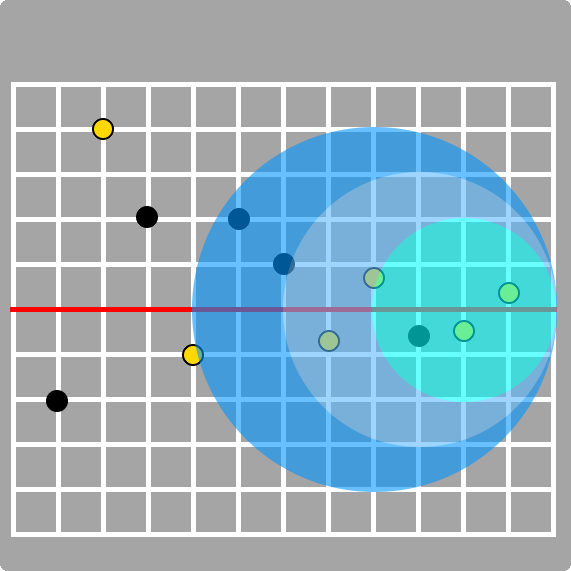
\includegraphics[scale=0.3]{Images/8.2.2.png}
    \end{figure}

    \newpage



    \begin{ltheorem}{\{$p_n$\} in compact space have
    \{$p_{n_k}$\} $\rightarrow$ p}{1.5cm}
        \item If \{$p_n$\} is a sequence in a compact metric space X,
            then some subsequence converges to p $\in$ X.

            \begin{proof}[15.5cm]
                Let E be the range of \{$p_n$\}.

                If E is finite, there is a p $\in$ E and sequence
                \{$n_k$\} with $n_k$ $<$ $n_{k+1}$ such that
                $p_{n_1}$ = $p_{n_2}$ = ... = p.
                Thus, \{$p_{n_k}$\} $\rightarrow$ p.

                If E is infinite, then by {\color{red} theorem 6.3.10},
                then there exists a p $\in$ E'.

                Then there are $n_k$ such that d($p_{n_k}$,p) $<$ $\frac{1}{k}$.
                Thus, \{$p_{n_k}$\} $\rightarrow$ p.                
            \end{proof}

        \item Every bounded sequence in $\mathbb{R}^k$ contains
            a convergent subsequence

            \begin{proof}[15.5cm]
                Let E be a bounded sequence in $\mathbb{R}^k$.
                Since E $\cup$ E' is bounded and closed, then by
                {\color{red} theorem 6.3.13}, E $\cup$ E' is compact.
                
                Thus by part a, E contains a convergent subsequence.
            \end{proof}
    \end{ltheorem}

    \vspace{0.5cm}



    \begin{wtheorem}{The set of subsequential limits is closed}{16cm}
        The subsequential limits of \{$p_n$\} in metric space X form
        a closed subset of X
    \end{wtheorem}
    
    \begin{proof}
        Let E be the range of the set of all subsequential limits of \{$p_n$\}.
        
        If E is empty, then E is closed.
        If E is finite, then E' is empty so E is closed.

        Suppose E is infinite. Then, let q $\in$ E'.

        Since q $\in$ E', there is a x $\in$ E where d(x,q) $<$ $\frac{\epsilon}{2}$.

        Since x $\in$ E, there is a \{$p_{n_k}$\} $\rightarrow$ x
        so there is a N such that for n $\geq$ N,
        d($p_{n_k}$,x) $<$ $\frac{\epsilon}{2}$.

        Thus, d($p_{n_k}$,q) $\leq$ d($p_{n_k}$,x) + d(x,q) $<$ $\epsilon$
        so q is a subsequential limit of \{$p_n$\}.
        
        Thus, q $\in$ E so E is closed.
    \end{proof}


        
    \begin{figure}[h]
        \centering
        
\includegraphics[scale=0.3]{Images/8.2.4.png}
    \end{figure}





\subsection{ Cauchy Sequences }

    \begin{definition}{Metric Spaces}{16cm}
        Sequence \{$p_n$\} $\in$ X is a {\color{lblue} Cauchy sequence} if:

        \hspace{0.5cm}
        For every $\epsilon$ $>$ 0, there is a N $\in$ $\mathbb{Z}$ such that
        for all n,m $\geq$ N, d($p_n$,$p_m$) $<$ $\epsilon$

        Let nonempty E $\subset$ X and S $\subset$ $\mathbb{R}$ of 
        d(p,q) where p,q $\in$ E.
        Let sup(S) = diam(E).

        If \{$p_n$\} $\in$ X, and $p_N, p_{N+1}, ... $ $\in$ $E_N$, then
        \{$p_n$\} is a Cauchy sequence if and only if
        $\lim_{N \rightarrow \infty}$ diam($E_N$) = 0.
    \end{definition}

    \newpage



    \begin{ltheorem}{Cauchy sequences and its closure have the same diam}{1.5cm}
        \item If $\overline{E}$ $\subset$ X, then diam($\overline{E}$) = diam(E).
        
            \begin{proof}[15.5cm]
                Since E $\subset$ $\overline{E}$, then
                diam(E) $\leq$ diam($\overline{E}$).

                For $\epsilon$ $>$ 0, let p,q $\in$ E'.

                Thus, there are p',q' $\in$ E such that
                d(p',p) $<$ $\epsilon$ and d(q',q) $<$ $\epsilon$.
                Thus:

                d(p,q) $\leq$ d(p,p') + d(p',q') + d(q',q)
                $<$ 2$\epsilon$ + d(p',q')
                $\leq$ 2$\epsilon$ + diam(E).

                Thus, diam($\overline{E}$) $\leq$ 2$\epsilon$ + diam(E)
                so diam($\overline{E}$) = diam(E).                
            \end{proof}

        \item For compact sets $K_n$ $\subset$ K where $K_{n+1}$ $\subset$ $K_n$
            and $\lim_{n \rightarrow \infty}$ diam($K_N$) = 0,
            then $\cap$ $K_n$ consist of only one point.

            \begin{proof}[15.5cm]
                Let K = $\cap$ $K_n$.
                Since $K_n$ is a sequence of compact sets, then
                by {\color{orange} corollary 6.3.8}, K is nonempty.

                If K contains more than one point, then diam(K) $>$ 0.
                But since K $\subset$ $K_n$, then diam(K) $\leq$ diam($K_n$)
                which contradicts that diam($K_n$) $\rightarrow$ 0.
            \end{proof}
    \end{ltheorem}

    \vspace{0.5cm}



    \begin{ltheorem}{Convergent sequences are cauchy sequences}{1.5cm}
        \item Every convergent sequence is a Cauchy sequence

            \begin{proof}[15.5cm]
                If $p_n$ $\rightarrow$ p and $\epsilon$ $>$ 0, there is a
                N such that for all n $\geq$ N, d(p,$p_n$) $<$ $\frac{\epsilon}{2}$.
                Thus, for m,n $\geq$ N:

				\hspace{0.5cm}
				d($p_n$,$p_m$) $\leq$ d($p_n$,p) + d(p,$p_m$) $<$ $\epsilon$.

				Thus, \{$p_n$\} is a Cauchy sequence.                
            \end{proof}

        \item If \{$p_n$\} is a Cauchy sequence in compact metric space X,
            then \{$p_n$\} converges to some p $\in$ X

            \begin{proof}[15.5cm]
                Let \{$p_n$\} be a Cauchy sequence in compact space X.

				Let	$p_N, p_{N+1}, ... $ $\in$ $E_N$.

				Since \{$p_n$\} is a Cauchy sequence, then
				$\lim_{N \rightarrow \infty}$ diam($\overline{E_N}$) = 0.
				Since $\overline{E_N}$ is closed in compact X, then
				by {\color{red} theorem 6.3.5}, $\overline{E_N}$ is compact.

				Since $E_{N+1}$ $\subset$ $E_N$, then $\overline{E_{N+1}}$
				$\subset$ $\overline{E_N}$ and thus, by
                {\color{red} theorem 8.3.2b},
				then there is a unique p $\in$ $\overline{E_N}$ for every N.

				Since p $\in$ $\overline{E_N}$, then d(p,q) $<$ $\epsilon$ for
                every q $\in$ $\overline{E_N}$ so every q $\in$ $E_N$.

                Then for $\epsilon$ $>$ 0, there is a $N_0$ such that
                for N $\geq$ $N_0$, diam($\overline{E_N}$) $<$ $\epsilon$.

				Thus, d($p_n$,p) $<$ $\epsilon$ for n $\geq$ $N_0$ so
                \{$p_n$\} $\rightarrow$ p.
            \end{proof}

        \item In $\mathbb{R}^k$, every Cauchy sequence converges
        
            \begin{proof}[15.5cm]
                Let \{$x_n$\} be a Cauchy sequence in $\mathbb{R}^k$.
				Let $x_N, x_{N+1}, ... $ $\in$ $E_N$.

				Then for some N, diam($E_N$) $<$ 1.
				Thus, the range of \{$x_n$\}
                = $E_N$ $\cup$ \{$x_1, ... , x_{N-1}$\}.
				Thus, \{$x_n$\} is bounded.

				Thus, the $\overline{\{x_n\}}$ is closed and bounded so by
                {\color{red} theorem 6.3.13}, $\overline{\{x_n\}}$ is compact.
				Thus, by part b, \{$x_n$\} converges to some
                p $\in$ $\mathbb{R}^k$.
            \end{proof}
    \end{ltheorem}

    \newpage


    
    \begin{definition}{Complete}{16cm}
        A metric space where every Cauchy sequence converges
        is {\color{lblue} complete}.

		Thus, by {\color{red} theorem 8.3.3}, all compact and Euclidean
		spaces are complete.
    \end{definition}
    
    \vspace{0.5cm}



    \begin{definition}{Monotonic Sequences}{16cm}
        A sequence \{$s_n$\} of real numbers is:
    \end{definition}

	\begin{enumerate}[label=(\alph*), leftmargin=2cm, itemsep=0.1cm]
		\item {\color{lblue} monotonically increasing} if $s_n$ $\leq$ $s_{n+1}$
		
		\item {\color{lblue} monotonically decreasing} if $s_n$ $\geq$ $s_{n+1}$
	\end{enumerate}

    \vspace{0.5cm}



    \begin{wtheorem}{Monotonic sequences converge if bounded}{16cm}
        Suppose \{$s_n$\} is monotonic. Then \{$s_n$\} converges if
		and only if it is bounded
    \end{wtheorem}
    
    \begin{proof}
        Suppose $s_n$ $\leq$ $s_{n+1}$.
        Let E be the range of \{$s_n$\}.
        
        Suppose \{$s_n$\} is bounded.
        
        Let s = sup(E) so $s_n$ $\leq$ s.
        For every $\epsilon$ $>$ 0, there is a N such that
        s - $\epsilon$ $<$ $s_N$ $\leq$ s
        else s-$\epsilon$ would be an upper bound of E
        which contradicts s = sup(E).

        Since \{$s_n$\} increases, then for n $\geq$ N,
        s - $\epsilon$ $<$ $s_N$ $\leq$ $s_n$ $\leq$ s
        so \{$s_n$\} $\rightarrow$ s.

        \vspace{0.2cm}

        Suppose \{$s_n$\} converges to s.

        Then for $\epsilon$ $>$ 0, there is a N such that for n $\geq$ N,
        s - $\epsilon$ $<$ $s_N$ $\leq$ $s_n$ $\leq$ s.

        Thus, \{$s_n$\} is bounded from above.

        \vspace{0.4cm}

        Suppose $s_n$ $\geq$ $s_{n+1}$. Let E be the range of \{$s_n$\}.

        Suppose \{$s_n$\} is bounded.

        Let s = inf(E) so $s_n$ $\geq$ s.
        For every $\epsilon$ $>$ 0, there is a N such that
        s $\leq$ $s_N$ $<$ s + $\epsilon$
        else s+$\epsilon$ would be a lower bound of E
        which contradicts s = inf(E).

        Since \{$s_n$\} decreases, then for n $\geq$ N,
        s $\leq$ $s_n$ $\leq$ $s_N$ $<$ s + $\epsilon$
        so \{$s_n$\} $\rightarrow$ s.

        \vspace{0.2cm}

        Suppose \{$s_n$\} converges to s.

        Then for $\epsilon$ $>$ 0, there is a N such that for n $\geq$ N,
        s $\leq$ $s_n$ $\leq$ $s_N$ $<$ s + $\epsilon$.

        Thus, \{$s_n$\} is bounded from below.
    \end{proof}	




